%%%%%%%%%%%%%%%%%%%%%%%%%%%%%%%%%%%%%%%%%%%%%%%%%%%%%%%%%%
%
% Vzor pro sazbu kvalifikační práce
%
% Západočeská univerzita v Plzni
% Fakulta aplikovaných věd
% Katedra informatiky a výpočetní techniky
%
% Petr Lobaz, lobaz@kiv.zcu.cz, 2016/03/14
%
%%%%%%%%%%%%%%%%%%%%%%%%%%%%%%%%%%%%%%%%%%%%%%%%%%%%%%%%%%

% Možné jazyky práce: czech, english
% Možné typy práce: BP (bakalářská), DP (diplomová)
\documentclass[czech,DP]{thesiskiv}

% Definujte údaje pro vstupní strany
%
% Jméno a příjmení; kvůli textu prohlášení určete, 
% zda jde o mužské, nebo ženské jméno.
\author{Zdeněk Valeš}
\declarationmale

%alternativa: 
%\declarationfemale

% Název práce
\title{Určování nahraditelnosti a\\kompatibility webových služeba}

% 
% Texty abstraktů (anglicky, česky)
%
\abstracttexten{The text of the abstract (in English). It contains the English translation of the thesis title and a short description of the thesis.}

\abstracttextcz{Text abstraktu (česky). Obsahuje krátkou anotaci (cca 10 řádek) v češtině. Budete ji potřebovat i při vyplňování údajů o bakalářské práci ve STAGu. Český i anglický abstrakt by měly být na stejné stránce a měly by si obsahem co možná nejvíce odpovídat (samozřejmě není možný doslovný překlad!).
}

% Na titulní stranu a do textu prohlášení se automaticky vkládá 
% aktuální rok, resp. datum. Můžete je změnit:
%\titlepageyear{2016}
%\declarationdate{1. března 2016}

% Ve zvláštních případech je možné ovlivnit i ostatní texty:
%
%\university{Západočeská univerzita v Plzni}
%\faculty{Fakulta aplikovaných věd}
%\department{Katedra informatiky a výpočetní techniky}
%\subject{Bakalářská práce}
%\titlepagetown{Plzeň}
%\declarationtown{Plzni}

%%%%%%%%%%%%%%%%%%%%%%%%%%%%%%%%%%%%%%%%%%%%%%%%%%%%%%%%%%
%
% DODATEČNÉ BALÍČKY PRO SAZBU
% Jejich užívání či neužívání záleží na libovůli autora 
% práce
%
%%%%%%%%%%%%%%%%%%%%%%%%%%%%%%%%%%%%%%%%%%%%%%%%%%%%%%%%%%

% Zařadit literaturu do obsahu
\usepackage[nottoc,notlot,notlof]{tocbibind}

% Umožňuje vkládání obrázků
\usepackage[pdftex]{graphicx}
\graphicspath{{./img/}}

% Odkazy v PDF jsou aktivní; navíc se automaticky vkládá
% balíček 'url', který umožňuje např. dělení slov
% uvnitř URL
\usepackage[pdftex]{hyperref}
\hypersetup{colorlinks=true,
  unicode=true,
  linkcolor=black,
  citecolor=black,
  urlcolor=black,
  bookmarksopen=true}

% Při používání citačního stylu csplainnatkiv
% (odvozen z csplainnat, http://repo.or.cz/w/csplainnat.git)
% lze snadno modifikovat vzhled citací v textu
\usepackage[numbers,sort&compress]{natbib}
%%%%%%%%%%%%%%%%%%%%%%%%%%%%%%%%%%%%%%%%%%%%%%%%%%%%%%%%%%
%
% VLASTNÍ TEXT PRÁCE
%
%%%%%%%%%%%%%%%%%%%%%%%%%%%%%%%%%%%%%%%%%%%%%%%%%%%%%%%%%%
\begin{document}
%
\maketitle
\tableofcontents

\chapter{Úvod}

- k čemu je práce dobrá
- co text práce obahuje
- use casy

\chapter{Principy webových služeb, techniky}

 - co je to API
 - co jsou to webové služby
 - REST

\chapter{Datové typy a porovnávání}

- přednášky z FJP
- jak jazyky řeší datové typy
	- rekurzivní vs. nerekurzivní
- primitivní typy (v xsd)
- built-in typy (v Jave)
- tady budu citovat \cite{abadi1995subytping}
	- subtyping: A <: B <=> A může být použito v kdekoliv kde je očekáváno B
	- kontravariance: F'(A) <: F(B) <=> B <: A

\subsection{Porovnávání datových typů}

 - jak to funguje
 - problémy při porovnání
 - subtyping vs. matching (\cite{abadi1995subytping})


\chapter{Popis ukládání metadat v CRCE, popis indexování API}

 - V této kapitole jsou popsány obecné způsoby ukládání metadat v CRCE
 - také jsou popsány podporované formáty API a způsoby jejich indexování

\section{Metadata v CRCE}

 - tady budu citovat \cite{brada2015repository}
 - Resource + Capability + Properties + Atributy
 	- stromová struktura
 - taky Requirements, ale ty v práci nepoužívám
 - Capabilita je rekurzivní + má napespace
 - Jsou root capability (přiřazené přímo Resource) a child capabilities
 - Capability mají Attributy + Properties
 - Properties mají atributy
 - Lze tak modelovat různé vlastnosti indexovaného objektu (viz \cite{brada2015repository}, tam je to dobře popsaný)
 
 \begin{figure}[h]
 	\centering
 	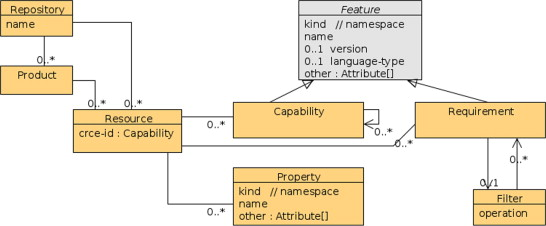
\includegraphics{resource-uml}
 	\caption{Reprezentace metadat v CRCE}
 	\label{fig:crce-resource-uml}
 \end{figure}

\section{Indexování API}

- různé druhy jsou jinak indexované
- každý druh API indexován vlastním modulem - diplomky Pejřimovského \cite{pejrimovsky2015ws} a Hessové \cite{hessova2015rest}
- někde by asi bylo fajn ustanovit názvosloví použité v práci:
	- co je API: interface přístupné skrze síť (internet)
	- co je web service: service popsaný WSDL, WADL, nebo Json-WSP dokumentem
	- co je service: Service element in WSDL
	- co je endpoint
		- WSDL: port+operation
		- endpoint: REST, WADL, JSON-WSP
- API je v CRCE uloženo jako Resource		
- popis API je reprezentován jako samostatná feature (1 root Capability) daného Resource
- Service a endpoint jsou reprezentovány jako Capaibility
- endpoint parametry, endpoint response, endpoint request body a endpoint request body jako Property
- vlastní hodnoty pak jako Attribute
- příklad metadat indexovaného API: \ref{fig:indexed-api-example}

 \begin{figure}[h]
	\centering
	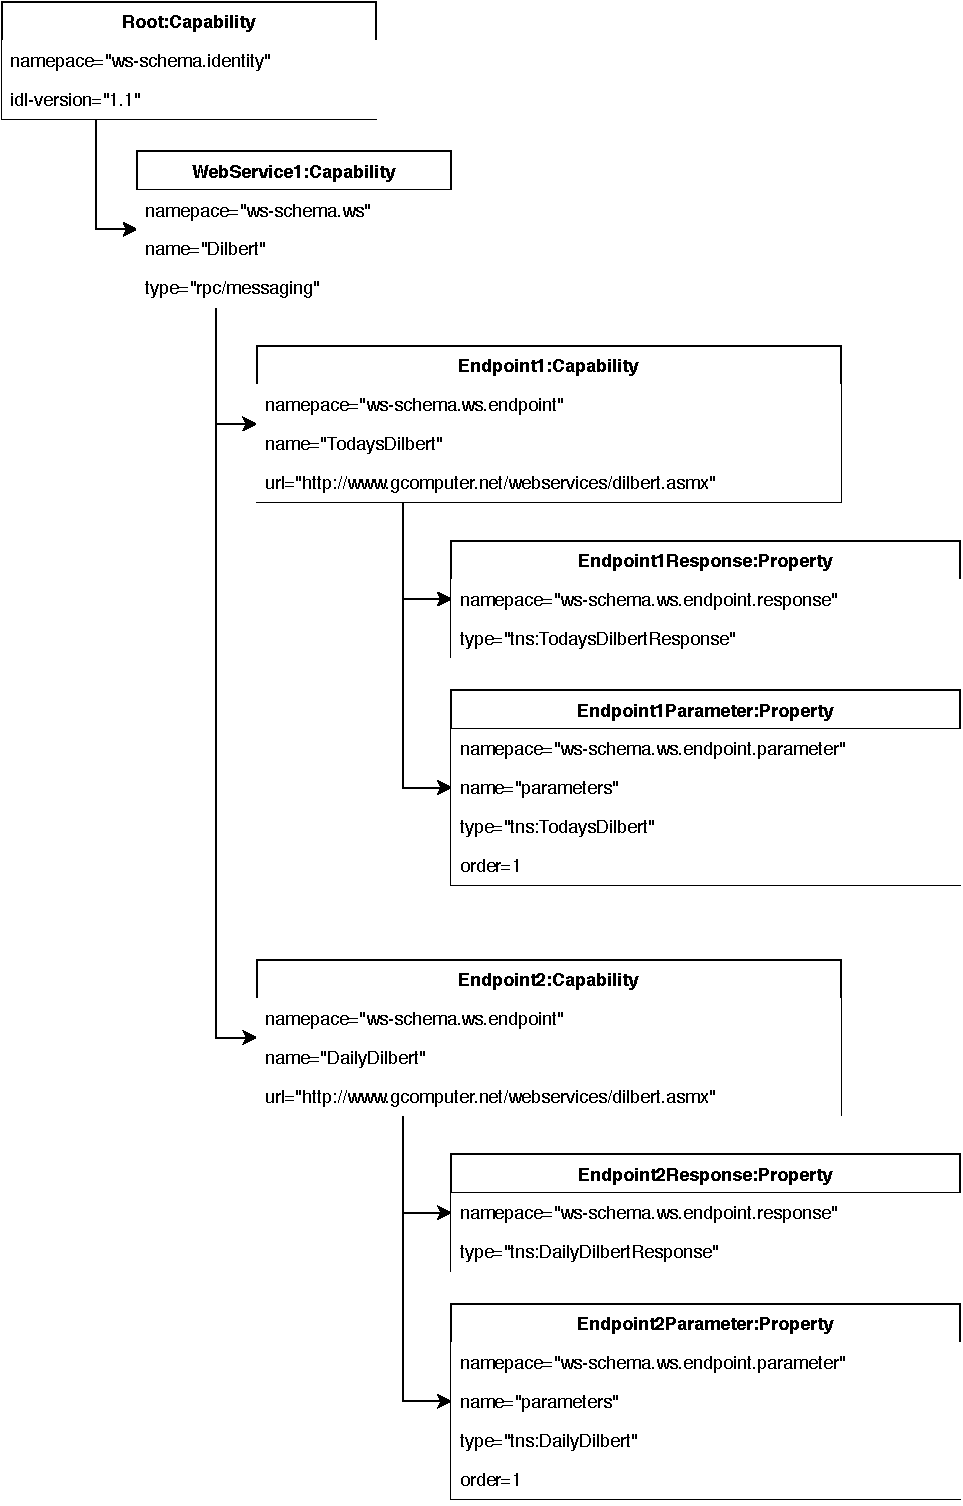
\includegraphics[height=13cm]{indexed-api-example}
	\caption{Příklad indexované SOAP web service Dilbert }
	\label{fig:indexed-api-example}
\end{figure}

\subsection{Indexování REST API}

- práce: \cite{hessova2015rest}
- binární analýza JAR s implementací API
- funguje na principu hledání patternů v byte kódu
- indexer vytváří hierarchii metadat ve formátu root capability -> child endpoint capabilities
- podpora formátů:
	- REST: JAX-RS, Spring Web MVC podporovány

\subsection{Indexování WS}

- práce: Pejřimovského \cite{pejrimovsky2015ws}
- nějaký trefný obrázek indexovaných dat
- konkrétní formát API detekován z buď z formátu vstupního souboru, nebo z metadata v top elementech
- podle typu je pak použit daný parser
- podpora formátů:
	- WSDL: hierarchie root capability -> web service capabilities -> child endpoint capabilities
	- WADL, Json-WSP: hierarchie root capability -> child endpoint capabilities
	- parsování souboru s popisem API, CRCE stačí i URL
- indexer obsahoval drobné chyby, které jsem v rámci DP opravil
	- špatná indexace URL v případě WSDL (nebyla podle specifikace)

\subsection{Limity indexování}

 - custom datové typy
 - 2 problémy
	- rekurzivní typy
		- jsou způsoby pro jejich rozvoj: \cite{abadi1995subytping} a ukládání
		- nicméně indexovací logika není implementovaná (ani v jednom ze zmíněných indexerů)
	- chybějící definice custom typů
		- v případě např REST jsou uloženy v implementaci (nemusí se jednat ani o stejnou knihovnu) a indexer k nim nemusí mít přístup
		- tím pádem je jméno datového typu (např. fully qualified name v případě Java třídy) jedinou informací, která je o typu dostupná

\chapter{Popis funkce porovnávače (co se jak porovnává pro jaké typy API)}

- zmínit taky omezení, která plynou z indexovaných dat
- v podstatě se porovnávají stromy Capabilit
- detaily v euromicro článku

\section{Popis porovnávacího algoritmu}
- WSDL porovnávač má v nejhorším možném případě složitost $O(n^3)$, závisí na počtu WS, a počtu endpointů ve WS 
- problémy řešené v algoritmu:
	1. jak vybrat který endpoint/ws porovnat s kterým
	2. MOV - pick the best
	3. datové typy (java built-in, xsd, custom)
	4. kontravariance (počkám a co řekne p. Brada)
	5. verze v URL u REST API (taky vede na MOV)
	
\subsection{MOV flag}	

- popsat MOV
- co: Příznak označující, že API/endpoint má (částečně) shodnou implementaci, ale nachází se na jiné adrese
- proč: endpointy v API mohou mít jiné url/jména, ale implementačně mohou být shodné -> potřeba detekovat
- jak: na základě ostatních metadat (počet parametrů, počet endpointů ve WS)

- nemusí vždy fungovat
- algorimuts:
	- obecná detekce před samotným porovnáním -> MovDetectionResult
		- 3x diff: host, path to endpoint, operace
	- MovDetectionResult se pak použije při výběru endpointu k porovnání a při samotném porovnání (pickBest)
	
- kombinace které vedou na mov: 
	- $h \land !pe \land !o$
	- $h \land pe \land !o$
	- todo
	- todo
	
	
\section{Výsledek porovnání - Diff}	
- popis výsledné datové struktury
	- Diff, Compatibility
	- vychází z \cite{brada2006diff}
	- stromová struktura rozdílů mezi jednotlivými uzly stromu metadat
	- obrázek \ref{fig:diff-construction} hezky popisuje jak to vznikne
	- výsledné hodnoty diffu a jejich významy pro klienta v tabulce \ref{tab:diff-level}
	
\begin{figure}[h]
	\centering
	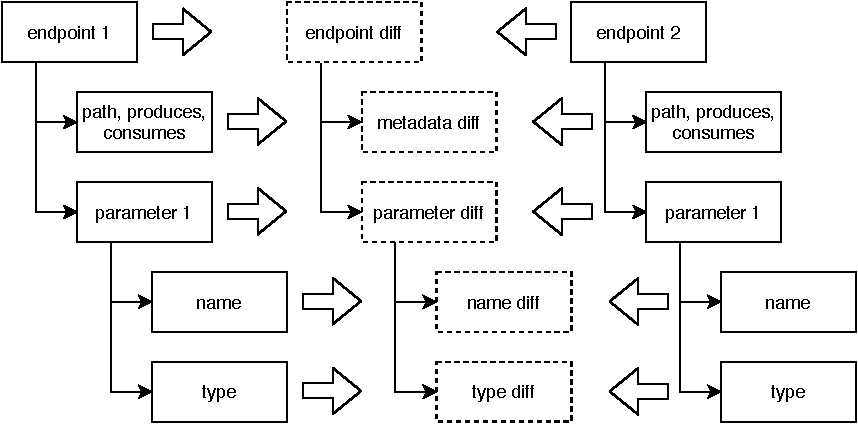
\includegraphics{diff-construction}
	\caption{Vytvoření diffů}
	\label{fig:diff-construction}
\end{figure}

\subsection{Vyhodnocení výsledku}

- jak probíhá vyhodnocení (nejdříve se určí hodnoty listů, z nich se pak počítá dál nahoru)

\begin{table}[h!]
	\centering
	\begin{tabular}{c|c}
		Difference type & Impact on client  \\
		\hline
		None (NON) & safe \\
		Generalization (GEN) & safe  \\
		Insertion (INS) & safe \\
		Deletion (DEL) & potentially dangerous \\
		Specialization (SPE) & potentially dangerous \\
		Mutation (MUT) & dangerous \\
		Unkown (UNK) & dangerous
	\end{tabular}
	\caption{Types of differences between two nodes }
	\label{tab:diff-level}
\end{table}

\chapter{Implementační detaily (jen stručně)}

 - zmínit, proč třídy pro porovnávání REST API a WS nemají společného předka (krom rozhraní)
 	- důvod: chtěl jsem nechat implementaci obou porovnávačů oddělenou pro případ, že by se změnila funkce indexerů

\chapter{Testování}

- nějaká reálná data
	- STAG (WSDL)
- i syntetická data
 
% 
% PRO ANGLICKOU SAZBU JE NUTNÉ ZMĚNIT
% CITAČNÍ STYL!
%
\bibliographystyle{csplainnatkiv}
{\raggedright\small
\bibliography{literatura}
}

\end{document}
